\documentclass[letterpaper]{article}
\usepackage[submission]{aaai2027}
\copyrighttext{Copyright \copyright\ 2027, Association for the Advancement of Artificial Intelligence (www.aaai.org). All rights reserved.}
\usepackage[hyphens]{url}
\usepackage{graphicx}
\urlstyle{rm}
\def\UrlFont{\rm}
\usepackage{natbib}
\usepackage{caption}
\usepackage{booktabs}
\usepackage{amsmath,amssymb}
\frenchspacing
\pdfinfo{/TemplateVersion (2027.1)}
\setcounter{secnumdepth}{2}
\title{OLIGARCH: \underline{OLI}gonucleotide \underline{G}eneration, \underline{A}ctive learning, \underline{R}epresentation Adaptation, and \underline{C}onstrained \underline{H}it Discovery}
\author{Anonymous Submission}
\affiliations{}
\begin{document}
\maketitle

\noindent\textbf{Code and Data Availability} --- The authors commit to open-sourcing all project code and releasing reproducibility materials upon acceptance. Third-party datasets will be linked under their original licenses.

\begin{abstract}
Oligonucleotide discovery requires prioritizing molecules and measurements under limited resources, yet predictive advances do not necessarily improve these decisions. We introduce OLIGARCH, a framework for evaluating adaptive molecular search and experimental decisions in oligonucleotide discovery. Two parallel environments support chemistry-constrained antisense oligonucleotide construction using frozen predictors and budgeted acquisition of recorded assay outcomes. Complementary studies examine representation adaptation, active learning, potency interpretation, concentration selection, and planning. Classical predictors remain stronger than the tested foundation-model adaptations, while uncertainty acquisition improves normalized prediction learning-curve area by 0.0095 across 40 Huesken splits. Bayesian updates reduce prediction error from 29.42 to 25.80 percentage points, but updated greedy selection finds more screen hits than the tested reinforcement-learning policy. Supervised molecular pretraining matches or exceeds subsequent reinforcement learning on six of eight development-stage targets with fewer offline predictor requests. Recognizing potency bounds increases credited discoveries without establishing a language-agent advantage. Retrospective fixed stopping reduces concentration readouts by 63.8\% and agrees with all 239 resolved reference labels. In a synthetic planning model, greedy is optimal in 108 of 162 settings and one-step rollout in 150. These findings connect predictive learning, evidence sufficiency, and planning opportunity to resource allocation. OLIGARCH supplies reusable tasks and controls for identifying where adaptive computation adds decision value.

\end{abstract}


\section{Introduction}
Oligonucleotides are short chains of deoxyribonucleic acid (DNA) or ribonucleic acid (RNA) whose sequences enable selective recognition of complementary nucleic acids. Antisense oligonucleotides (ASOs) are single-stranded molecules that bind complementary RNA to change its abundance or processing. This sequence-directed intervention makes them useful for probing gene function and developing therapies: early antisense experiments demonstrated sequence-specific inhibition of viral replication \citep{zamecnik}, while nusinersen demonstrated therapeutic benefit in infantile-onset spinal muscular atrophy by modifying splicing, the process that joins selected RNA segments \citep{finkel}. Turning this programmability into effective molecules requires choosing sequences, chemical modifications, and informative experiments.

Discovery requires choosing molecules, screens, and follow-up measurements. Predictions depend on chemistry, the target RNA transcript (a gene's RNA copy), delivery, cell system, dose, and response. Limited resources motivate selective measurement, yet predictive accuracy alone does not ensure effective decisions.

Three objectives guide the framework. \emph{Prediction} estimates an experimental outcome, also called an endpoint. \emph{Molecular design} searches for valid structures using a \emph{surrogate}: a predictive model that stands in for an expensive experiment. \emph{Experimental selection} chooses which laboratory tests, or assays, to acquire. A \emph{policy} is the rule that makes these choices. Better prediction need not find more successful candidates, or \emph{hits}; high surrogate scores need not identify effective molecules. These distinctions motivate evaluating each decision directly.

OLIGARCH implements two parallel environments using OligoGym and ASO Atlas 2.0. Molecular design constructs ASOs complementary to a transcript and charges for each call to a \emph{frozen} predictor, whose parameters stay fixed during search. Experimental selection charges to reveal a historical assay result, then updates predictions using that measurement. A \emph{greedy} policy selects the currently highest-ranked option. Bayesian methods update probabilities as evidence arrives; lookahead considers how a choice could affect later decisions.

Reinforcement learning (RL) trains policies to maximize rewards over a sequence of decisions \citep{sutton}. We use proximal policy optimization (PPO), a standard policy-learning algorithm \citep{ppo}, to ask four questions: do learned representations and selective measurement improve prediction; does PPO add value beyond supervised pretraining; do learned assay selectors improve on greedy and Bayesian controls; and how do potency definitions and stopping rules change measurement efficiency? We contribute two ASO decision environments with explicit chemical validity, information access, and expenditure; comparisons assessing representation learning, policy initialization, and sequential planning; and potency-evidence studies that test what measurements suffice for a decision. These contributions guide allocation of modeling and experimental effort.

\section{Related Work}
Adaptive decision-making for targeted oligonucleotide discovery remains underexplored, motivating systematic evaluation of how predictive models guide molecular design and experimental choices \citep{oligoai,oligorl,oligogym}.

\paragraph{Oligonucleotide prediction and design.}
OligoGym provides endpoint-specific prediction benchmarks \citep{oligogym}. OligoAI models ASO efficacy from sequence, chemistry, target context, and dose \citep{oligoai}; ASOptimizer studies chemistry-aware ASO design for IDO1 regulation \citep{asoptimizer}. For small interfering RNA (siRNA), OligoFormer combines thermodynamic features with representations from an RNA foundation model (RNA-FM) \citep{oligoformer,rnafm}. Low-rank adaptation (LoRA) provides a parameter-efficient way to adapt pretrained models \citep{lora}. OLIGARCH evaluates how these predictive approaches inform budgeted decisions across distinct endpoints.

\paragraph{Budgeted molecular search.}
OligoRL applies reinforcement learning to constrained oligonucleotide pools, including barcodes and primers \citep{oligorl}. The Practical Molecular Optimization benchmark emphasizes the number of scoring-model calls needed to optimize molecules and the importance of established baselines \citep{pmo}. Our molecular environment combines transcript-complementary ASO construction with explicit chemistry rules and applicability-aware scoring. We separate the contribution of supervised initialization from subsequent PPO refinement and account for predictor requests during both preparation and deployment.

\paragraph{Experimental acquisition and planning.}
GeneDisco benchmarks active learning on recorded biological experiments \citep{genedisco}. Nonmyopic active search considers future discoveries, while multifidelity search combines measurements of different costs and informativeness \citep{jiang,nguyen}. OLIGARCH brings these questions to linked ASO screening and potency assays, where purchased outcomes determine follow-up eligibility. Atlas also provides pipeline cost and strategy analyses \citep{atlas}. Our emphasis is sequential access to purchased outcomes, attribution of policy gains, and exact planning comparisons under a specified model.

\paragraph{Potency evidence and concentration choice.}
Guidelines distinguish absolute from relative half-maximal inhibitory concentrations ($\mathrm{IC}_{50}$) and specify when numerical estimates are supportable \citep{sebaugh}. Optimal dilution design studies concentration ranges and replication for potency estimation \citep{donev}. COBALT develops Bayesian learning and acquisition for censored measurements, which provide bounds instead of exact values \citep{cobalt}. Our contribution is an ASO-specific assessment of how qualified bounds change discovery credit and whether sequential measurements can resolve a potency threshold efficiently. We compare adaptive choices with fixed early stopping and separately assess decision agreement and curve quality.

\section{Methodology}
\subsection{Framework, Data, and Information Boundaries}
OligoGym supplies oligonucleotide datasets and published prediction baselines \citep{oligogym}. Its Huesken benchmark contains 2,431 measurements across 30 targets for small interfering RNA (siRNA), a distinct class of gene-silencing molecules. We keep this prediction task separate from ASO assays. The pinned ASO Atlas 2.0 release contains 295,007 readouts, 430 named targets, and 606 patents, with tables for inhibition, dose response, and toxicity in the nervous system and liver \citep{atlas}. Readouts can share compounds or experimental sources.

Each candidate retains its base sequence, sugar and backbone modifications, assay conditions, and source identity. Cleaning preserves measured values and units. Compatibility checks keep different chemistries and endpoints separate: inhibition percentage, potency in concentration units, and toxicity scores are not interchangeable.

Data roles distinguish predictor fitting, policy development, uncertainty calibration, and final assessment. A private measurement store, called the \emph{oracle}, reveals an outcome only when a policy pays for it. Separate \emph{sentinel} examples are never acquired and measure prediction error without affecting decisions. Molecular search instead queries a fixed set of endpoint models. Logs record every purchase or predictor request and its cost. These controls prevent access to unpurchased outcomes within a run; prior use of a dataset is reported separately.

\subsection{Prediction and Representation Learning}
Classical predictors include Ridge regression (linear regression with a penalty on large coefficients), random forests (RFs; ensembles of decision trees), Gaussian processes (GPs; probabilistic predictors), and convolutional neural networks (CNNs; models of local sequence patterns). Dataset-specific features and splits follow the benchmark reproduction. Chemistry-aware models include modification features; efficacy and toxicity are predicted separately.

For learned features, the RNA foundation model (RNA-FM) converts sequences into numerical vectors using a pretrained encoder \citep{rnafm}. In Huesken, we average nucleotide vectors within each strand and combine the two strands' features. Controls use \emph{one-hot} base indicators, frozen RNA-FM features with Ridge, or a frozen encoder with a trainable prediction head. Low-rank adaptation (LoRA) updates small rank-four matrices in the encoder's attention layers while keeping its original parameters fixed \citep{lora}. The Atlas study also supplies chemistry and assay features. Its classical control adds a target-specific offset to source-trained Ridge predictions.

Uncertainty has different meanings across models: RF spread measures disagreement between trees, whereas GP variance describes uncertainty under a probabilistic model. For online assay learning, a Bayesian linear correction updates a fixed source prediction $f_0$:
\begin{equation}
 \begin{gathered}
 y_i=f_0(x_i)+\phi_i^\top w+\epsilon_i,\\
 w\sim\mathcal N(0,\Lambda_0^{-1}),\quad
 \epsilon_i\sim\mathcal N(0,\sigma^2).
 \end{gathered}
 \label{eq:belief}
\end{equation}
Here $y_i$ is the measured response, $\phi_i$ is a feature vector, $w$ contains correction weights, and $\epsilon_i$ represents unexplained variation. $\mathcal N$ denotes a normal distribution. For acquired features $\Phi_t$, the inverse covariance (precision) becomes $\Lambda_t=\Lambda_0+\sigma^{-2}\Phi_t^\top\Phi_t$. Uncertainty about the predicted mean is $\phi^\top\Lambda_t^{-1}\phi$; adding $\sigma^2$ gives uncertainty about an observed response. 

\subsection{Active Learning}
\emph{Active learning} chooses which examples to measure next to improve prediction. Each round reveals a batch of labels (measured outcomes), refits the predictor on acquired labels, and evaluates on a fixed hidden test set. Random selection samples without replacement. Diversity selects sequences far from those already chosen. Uncertainty selects examples with the greatest model uncertainty. The hybrid diversifies within a shortlist of uncertain examples. Initial labels and internal validation labels count against the same budget.

We measure prediction with Pearson correlation $r$, which describes linear association between predicted and observed responses. The normalized area under the learning curve (AULC) integrates $r$ over acquired-label count and divides by the budget range: it summarizes prediction quality across budgets. We also evaluate how many labels are needed to reach a fixed accuracy threshold.

\subsection{Experimental-Selection Environment}
Each experimental-selection episode is one simulated campaign. Its state contains a fixed candidate pool, predictions and their uncertainty, available assays, purchased results, and remaining budget. A legal action purchases an unrevealed assay or stops. The oracle returns only that assay's recorded outcome; the policy then updates its belief. Missing measurements remain unavailable. With assay cost $c(a)$ and budget $B$, policies maximize expected newly established hits subject to $\sum_t c(a_t)\leq B$.

The single-dose task purchases inhibition measurements using either a frozen source predictor or the acquired-only Bayesian update in Equation~\ref{eq:belief}. A new purchase earns one unit when measured inhibition is strictly above 80 percentage points. Initial measurements consume budget but receive no new-hit credit. Greedy selects the highest current predicted mean; other controls use the fixed source ranking, uncertainty, or diversity. The expert-action PPO policy chooses among acquisition rules, such as highest predicted response, which then select a candidate. An action mask removes unavailable purchases \citep{ppo,masking}.

The linked-assay task couples an initial screen to a dose-response curve, which measures inhibition at several concentrations. A screen above 80\% unlocks the curve purchase. Absolute $\mathrm{IC}_{50}$ is the concentration producing 50\% inhibition; lower values indicate greater potency. A confirmed hit requires a paid, usable, in-range $\mathrm{IC}_{50}\leq500$ nanomolar (nM). Curve quality control (QC) requires at least four distinct positive finite doses, a 50\% crossing, sufficient response range, and fit $R^2>0.5$, where $R^2$ measures agreement with the observed responses. Modeled costs are \$500 per screen and \$2,000 per curve within a \$15,000 campaign.

Policies include PPO choosing candidate--assay pairs directly, PPO adjusting a baseline policy, greedy, and Bayesian lookahead. \emph{Nonmyopic} planning considers consequences beyond the next reward: lookahead evaluates possible observations and estimates later choices using a simpler policy \citep{jiang,nguyen}. Qwen language-model agents instead select among up to six proposals generated by candidate rankers. This smaller menu differs from full action access. Reported empirical comparisons use the verified single-dose replays and the separately frozen potency pilot; original linked-assay policy records are unavailable and their numerical summaries are excluded.

\subsection{Molecular-Design Environment}
The molecular task constructs ASOs against a specified transcript region. Its state contains target features, the unfinished molecule, remaining budgets, and an archive of scored candidates. A construction grammar---rules for valid molecules---organizes decisions as follows:
\begin{center}
\texttt{NEW $\to$ LENGTH $\to$ SITE $\to$ LAYOUT}\\
\texttt{$\to$ PATTERN $\to$ TERMINAL $\to$ COMMIT}.
\end{center}
The stages choose length, binding site, chemical layout and modification pattern, then finalize and submit the molecule. Its sequence complements the chosen transcript window. Action masks enforce validity and prevent repeated scoring. Only complete candidates call the predictors: constructing one molecule takes several decisions but consumes one scoring request.

Let $e(x)$ indicate whether molecule $x$ passes the fixed computational screens. Its utility $u(x)\in[0,1]$ is the predicted efficacy score on a fixed training-reference scale. For archive $A$, best eligible utility and reward are
\begin{align}
 Q(A)&=\max\bigl(\{0\}\cup\{u(x):x\in A,e(x)=1\}\bigr),\label{eq:archive}\\
 r_t&=Q(A_{t+1})-Q(A_t).\label{eq:reward}
\end{align}
An action earns reward only when it improves the best eligible score. Summing these rewards gives the total archive improvement; repeated scores earn no extra bonus. Required screens and advisory predictions remain separate, and unsupported endpoints stay unknown.

Supervised pretraining teaches a policy from scored examples before RL begins. Frozen models label valid candidates from training campaigns. A multilayer perceptron (MLP), a feed-forward neural network, takes positional sequence and chemistry features and predicts eligibility and utility. For $N$ examples with targets $(e_i,u_i)$, the loss combines binary cross-entropy (BCE) for eligibility with squared error for utility:
\begin{equation}
 \mathcal L_{\rm pre}=\frac1N\sum_i\left[
 \operatorname{BCE}(\hat e_i,e_i)+(\hat u_i-u_i)^2\right].
 \label{eq:pretraining}
\end{equation}
The predictions $(\hat e_i,\hat u_i)$ are bounded between zero and one by sigmoid functions. A pretrained policy can either choose successive construction steps or rank complete candidates directly. We compare both with PPO refinement using the same grammar and action masks \citep{ppo,masking}. The attribution comparison uses random, greedy, pretrained staged search, and PPO. All complete scored proposals, including the starting molecule, consume deployment budget. Offline pretraining, PPO, and checkpoint-selection requests are counted separately.

\subsection{Potency Evidence, Stopping, and Planning}
A potency result is \emph{censored} when the tested concentrations establish a bound rather than an in-range estimate. If inhibition already exceeds 50\% at the lowest dose, the absolute $\mathrm{IC}_{50}$ can be at or below that dose, assuming the response increases with concentration and passes QC. Such an upper bound can establish a potency threshold without locating the exact crossing. Lower bounds can similarly rule out potency. Curves whose bounds do not resolve the threshold, or that fail QC, remain inconclusive. Absolute 50\% inhibition differs from half of a curve's own maximum response.

Concentration selection reveals one recorded dose at a time, then either continues or classifies the ASO as potent, nonpotent, or inconclusive. The full-grid reference uses every dose and checks response validity and approximate monotonicity (inhibition increasing with concentration). Fixed early stopping starts near the potency threshold and stops when purchased values resolve the decision. Bayesian information gain chooses doses that reduce uncertainty about the response curve. Decision-aware selection instead reduces expected error in the potent/nonpotent decision. Both use candidate Hill curves (S-shaped dose responses) and development-selected confidence thresholds.

A separate synthetic study measures \emph{planning headroom}: the improvement available over greedy under a specified model \citep{jiang,nguyen}. Four candidates form two independent pairs, with linked outcomes within each pair. The belief assigns probabilities to all 16 positive/negative outcome combinations. A noisy screen supplies information; perfect confirmation reveals an outcome and rewards a hit. Confirmation can be bought directly, unlike in the linked-assay replay. Dynamic programming solves every reachable state to obtain the best expected yield under this model, called the \emph{Bayes-optimal} value \citep{sutton}:
\begin{equation}
 \begin{aligned}
 G(s,a)&=\sum_o P(o\mid s,a)[r(s,a,o)+V^*(s')],\\
 V^*(s)&=\max\{0,\max_{a\in\mathcal A(s)}G(s,a)\}.
 \end{aligned}
 \label{eq:dp}
\end{equation}
Here $s$ contains the belief and budget, $a$ is an affordable action, $o$ is its possible outcome, and $s'$ is the resulting state. $G$ combines immediate reward $r$ with future value $V^*$; stopping gives zero additional reward. The calculation averages over hidden outcomes rather than assuming they are known. One-step Bayesian rollout evaluates the next action and follows greedy thereafter. Greedy, rollout, random, and PPO receive the same information.

\section{Experimental Setup}
\paragraph{Prediction and acquisition.}
The reproduction study compares seven published best-performing efficacy models with a prespecified tolerance of $\pm0.03$ in Pearson correlation. The Huesken GP acquisition study uses 40 fresh random seeds controlling data splits after a separate exploratory pilot, with the benchmark's sequence-clustered train/test partitions, 50 initial labels, batches of 50, and a 1,000-label cap. The hybrid diversifies within the 200 most uncertain candidates. Its prespecified primary test is the paired uncertainty-minus-random AULC contrast; secondary comparisons use Holm correction to account for multiple tests. Five separate Huesken LoRA splits use nested 50/100/200-label budgets and acquired-only model selection. Atlas adaptation uses 2,869 or 4,781 source rows, including internal validation, and 200 target labels on F7, STAT3, and NLRP3. Source compositions and some validation memberships change, so this is not a controlled sample-size scaling curve.

\paragraph{Assay acquisition.}
The single-dose acquisition protocol fits the initial predictor on 12,000 rows and calibrates on 2,500 separate rows. Policy training uses F7/NLRP3/STAT3, development uses DMPK/PLN, and final replay uses DUX4/KCNQ2/PSD3/PTBP1/SMAD7. Exact target, patent, sequence, and compound checks separate roles; broader homology and patent-family independence remain unverified. Each replay pays for 10 shared initial and 40 new assays. A later diagnostic standardizes eligible pool size to 600 on PSD3 and SMAD7, using five policy seeds and five paired replay seeds. Its PPO action-selection and value-estimation networks each have three 32-unit hidden layers and train for 8,192 decisions per seed. These previously exposed targets are not fresh confirmation cohorts.

\paragraph{Molecular search.}
The tested grammar allows three 18- or 20-base designs with $2^{\prime}$-O-methoxyethyl (MOE) sugar modifications. Each of five policy seeds receives 576 surrogate-labeled examples over permitted training campaigns, followed by 20 passes through those examples. The MLP uses two 64-unit hidden layers and two prediction outputs. It minimizes Equation~\ref{eq:pretraining} with the Adam optimizer, learning rate $10^{-3}$, and batches of at most 64. PPO receives 16,384 construction decisions per seed, with equal weighting of rewards across time and at most 160 construction steps per episode. The principal deployment limit is eight requests including the starting molecule; 32 requests is a separate extrapolation condition. Saved model versions are selected using CFB. The eight reported targets mix training, checkpoint validation, and development roles, as retained in Table~\ref{tab:molecular}.

\paragraph{Potency and planning.}
The separately specified Qwen2.5-3B pilot buys complete dose panels (all recorded concentrations for one ASO), with an eight-panel cap including two starts, three seeds, and a primary 100 nM threshold. It contains 24 F7, 24 STAT3, and 15 NLRP3 panels and is not a rerun of the 500 nM linked-assay task. The concentration study uses 93 development ASOs (F7/STAT3) and 240 frozen assessment ASOs: 48 each from AGT, DNM2, KRAS, PCSK9, and TMPRSS6. Its seven patent groups are separated within this study, not certified as globally unseen. At 500 nM, assessment references comprise 108 potent, 131 nonpotent, and one unresolved panel. The Bayesian dose model assigns probabilities to 1,500 Hill curves and assumes normally distributed observation error with standard deviation 10 percentage points. Prespecified qualification requires false-positive and false-negative rates at most 5\%, decisions on at least 95\% of resolved references, and classifications of at most 5\% of unresolved references. Decision coverage may fall by no more than two percentage points relative to the baseline.

The planning grid crosses uncertainty settings $\{0.1,0.5,1\}$, confirmation costs $\{2,3,4\}$, budgets $\{4,6,8\}$, hit prevalences (expected fractions of positives) $\{0.25,0.5,0.75\}$, and pair-dependence mixture weights $\{0,0.75\}$. Screen cost is one; it correctly identifies positive and negative outcomes with probability 0.9 each. This yields 162 model settings. Increasing uncertainty brings candidates' initial hit probabilities closer to the same population mean. PPO uses three seeds with 32,768 decisions each on this same grid, not held-out task generalization.

\paragraph{Evidence and statistics.}
Prediction metrics are Pearson correlation and root-mean-square error (RMSE), which measures error in the original response units and weights large errors more strongly. Decision metrics are AULC, new hits, best eligible utility, and readouts per ASO. Methods share candidate pools and budget definitions within each comparison; different studies are not pooled into one effect. Replay seeds and availability draws are not independent biological replicates. We average within each target first, then weight targets equally. Frozen assessment outcomes are not used to repair failed stopping rules. Numerical claims are tied to preserved reports or saved aggregates. Historical linked-assay summaries lacking original records are excluded.

\begin{figure*}[t]
\centering
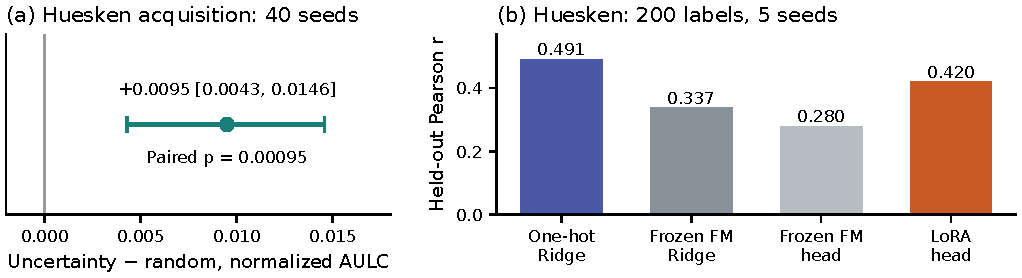
\includegraphics[width=\textwidth]{figures/prediction.pdf}
\caption{Prediction studies remain separate. AULC: normalized area under the learning curve; FM: RNA foundation model. (a) Prespecified Huesken uncertainty-acquisition effect with a 95\% confidence interval from resampling paired results across 40 data-split seeds. (b) Mean Huesken correlation at 200 acquired labels in a different five-seed representation study; bars are descriptive means. LoRA improves its matched frozen-head control but not one-hot Ridge.}
\label{fig:prediction}
\end{figure*}

\section{Results}
\subsection{Predictive Modeling and Active Learning}
We first test whether representation learning and selective measurement improve the predictive foundation used to guide decisions. Four of seven classical efficacy reproductions meet the prespecified tolerance; three remain unresolved. Figure~\ref{fig:prediction} compares acquisition and representation learning under their respective protocols.

On the 40 fresh Huesken seeds, uncertainty improves normalized Pearson AULC over random by $0.0095$ (bootstrap 95\% confidence interval $[0.0043,0.0146]$; paired $p=0.00095$). The hybrid improves it by $0.0112$ (Holm-adjusted $p=0.0026$); diversity's $0.0068$ improvement does not survive correction ($p=0.10$). These are within-dataset split results, not 40 independent biological studies. Uncertainty's estimated 72.5-label saving has interval $[-6,151]$ and adjusted $p=0.24$. No comparison at an individual label budget remains significant after correction for multiple tests. Thus, a modest average accuracy gain is supported, while significant threshold-based label savings and superiority over the other nonrandom policies are not.

At 200 Huesken labels, LoRA reaches mean Pearson $r=0.4196$, improving on its matched frozen-head control ($0.2801$), but remaining below one-hot Ridge ($0.4910$). Frozen RNA-FM with Ridge reaches $0.3374$. LoRA trails one-hot Ridge in learning-curve area on all five splits. On Atlas target adaptation, Ridge plus offset achieves RMSE 19.883/19.656 percentage points at the two source allocations, versus 22.391/22.340 for LoRA, under target adaptation with three passes through the training data. These comparisons support retaining inexpensive classical predictors as controls when adapting representations to limited-label tasks. LoRA improves its matched neural control, but architecture alone does not determine which predictor merits deployment.



\subsection{Experimental-Selection RL}\label{sec:expresults}
We then ask whether learning from purchased measurements translates into more discoveries. In the five-target online assay-learning study, Bayesian updating reduces never-acquired sentinel RMSE from 29.42 to 25.80 percentage points on identical PPO purchase trajectories. The fixed-kernel GP residual reference reaches 25.76. However, prediction intervals include the observed responses more often than their stated probability implies, and RMSE does not improve monotonically with more purchases. Better average prediction does not establish calibrated uncertainty.

Discovery favors updated greedy over PPO: 9.20 versus 8.36 mean new hits, compared with 3.76 for random. The online-learning PPO policy selects the frozen-source expert on all 1,000 final acquisition decisions. Thus, its improvement over random comes from following the fixed ranking rule. The later 600-candidate diagnostic reinforces this result (Table~\ref{tab:assays}). PPO chooses either the updated ranking (75.3\% of decisions) or the frozen source ranking (24.7\%). All methods find zero new hits on SMAD7; a post hoc audit finds four qualifying hits in its pool, compared with 185 on PSD3. The contrast highlights the importance of hit prevalence and ranking quality; two target groups cannot establish a general policy advantage. This separates the benefit of updating predictions from the incremental value of a learned acquisition policy.

\begin{table}[t]
\centering
\begin{tabular}{lrrr}
\toprule
Policy & PSD3 & SMAD7 & Mean\\
\midrule
Updated greedy &18.00&0.00&9.00\\
Expert-action PPO &17.92&0.00&8.96\\
Frozen source ranking &16.80&0.00&8.40\\
Random &13.40&0.00&6.70\\
\bottomrule
\end{tabular}
\caption{Verified 600-candidate diagnostic: new measured screen hits after 10 initial and 40 additional purchases. PPO averages five training seeds; replay seeds share two previously exposed target campaigns. These are single-dose hits, not potency confirmations.}
\label{tab:assays}
\end{table}

\subsection{Potency Adjudication and Measurement Efficiency}
We next test whether discovery counts change because of better selection or a more informative interpretation of purchased evidence. The source-audited F7 pilot isolates this distinction. At its frozen 100 nM cutoff, upper-bound qualification expands the eligible pool from six to eight of 24 panels. Mean new credited hits for greedy, random, and Qwen each change from 1.667 to 2.000. Evaluating both acquisition trajectories with the same bound-aware rule yields no gain for these methods. Thompson sampling, which chooses according to sampled hit probabilities, remains at 0.333 credited hits in the matched comparisons. Under the common bound-aware evaluator, changing its feedback rule reduces yield by 0.333 hits. STAT3 and NLRP3 contain no qualifying panels at this threshold. Adjudication recovers evidence without establishing a Qwen selection advantage.

Table~\ref{tab:dose} and Figure~\ref{fig:measurement} show the concentration study. Fixed early stopping uses 1.592 readouts per ASO versus 4.400 for the full grid, a 63.8\% reduction, with zero false positives or negatives against the 239 resolved references. Bayesian information gain also makes no resolved-reference errors but uses 2.817 readouts. Decision-aware selection uses 1.683 and makes one false positive and two false negatives. Its measurement count is 5.8\% higher than fixed stopping. Inconclusive rates are zero for early methods and $1/240$ for the full grid.

Crucially, \emph{all three early-stopping methods fail the prespecified unresolved-panel criterion}: each asserts a class on the one failed-QC reference. That panel includes a response outside the permitted raw range at an unpurchased dose. Evidence from the doses measured so far does not certify the quality of the whole curve. Consequently, the experiment does not establish its primary qualified measurement-reduction claim, despite the substantial descriptive saving. No assessment-dependent repair is applied. An exploratory TMPRSS6 contrast favors decision-aware stopping (1.208 versus 2.417 readouts, with no observed resolved-reference errors), but does not isolate adaptive ordering from the stopping rule or overturn the overall result.

\begin{table}[t]
\centering
\begin{tabular}{lrrr}
\toprule
Protocol &Readouts&FP/FN&Unknown\\
&&&assertions\\
\midrule
Full grid&4.400&0/0&0/1\\
Fixed stopping&1.592&0/0&1/1\\
Information gain&2.817&0/0&1/1\\
Decision-aware&1.683&1/2&1/1\\
\bottomrule
\end{tabular}
\caption{Frozen 240-ASO assessment. FP/FN: false positives/false negatives against 239 resolved references. The last column counts decisions made on the one unresolved panel, where the method should remain inconclusive. All early methods fail that QC criterion. Full-grid agreement is by construction, not independent ground truth.}
\label{tab:dose}
\end{table}

\subsection{Value of Nonmyopic Planning}
To quantify how much improvement a sequential policy could attain, we solve a small decision model exactly. Dynamic programming achieves mean expected yield 1.298591 over the 162 equally weighted synthetic settings. One-step Bayesian rollout reaches 1.296469, greedy 1.260482, PPO 1.241975, and random 0.691171. Greedy is optimal in 108 settings and rollout in 150; the largest optimal-minus-greedy gap is 0.400 expected discoveries. These are model expectations, not measured ASO hit counts or a significance test over biological replicates.

The prespecified slice in Figure~\ref{fig:measurement} shows headroom increasing with the uncertainty setting at a confirmation/screen cost ratio of four, while remaining zero at the two lower ratios. This is conditional on its budget, prevalence, and dependence assumptions, not a universal monotonic cost law. The study establishes that limited planning headroom can coexist with available gains in particular regimes. Its prior is not calibrated to Atlas and its direct-confirmation rule differs from the linked-assay task, so transferring these conditions to real campaigns remains an empirical question. PPO's failure to exploit the available gap also leaves optimization and representation limitations open.

\begin{figure*}[t]
\centering
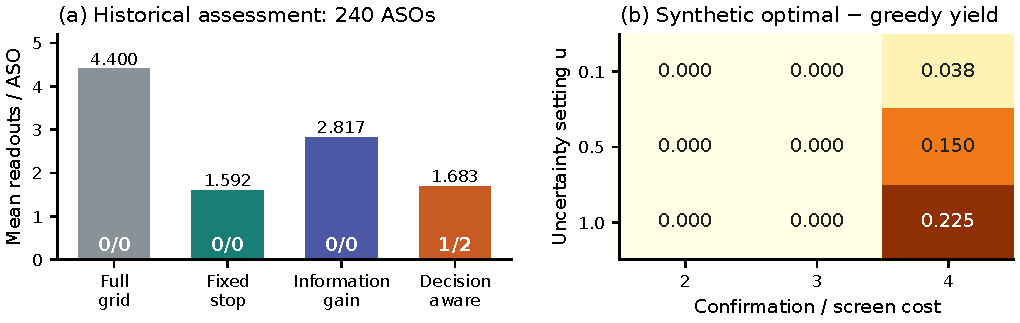
\includegraphics[width=\textwidth]{figures/measurement_planning.pdf}
\caption{Two distinct evidence settings. (a) Retrospective concentration measurements; labels inside bars count false positives/false negatives. Every early method classifies the unresolved reference and fails full-curve QC (Table~\ref{tab:dose}). (b) Model-based planning headroom for budget six, prevalence 0.5, and dependence-mixture weight 0.75. Cells show expected optimal-minus-greedy discoveries in the four-candidate synthetic model, not empirical ASO gains.}
\label{fig:measurement}
\end{figure*}

\subsection{Molecular-Design RL}
The parallel molecular task tests whether learning a search policy improves candidate proposals under a fixed scoring budget. The environment enforces its construction grammar and records the best eligible score after each request. Figure~\ref{fig:molecular} shows progress with each paid predictor request on the four original development targets. Table~\ref{tab:molecular} retains all eight reported targets and their exposure roles. Pretraining followed by staged construction matches or exceeds PPO on six of eight; PPO improves on CFB, used for checkpoint selection, and slightly on newly assessed APOC3. Greedy narrowly leads on F9. F12 remains zero because all 89 legal candidates fail the unchanged computational risk screen. The zero is retained without threshold tuning.

Across the four original development targets, PPO minus staged pretraining is $-0.006283$ utility at eight requests and $+0.006283$ at 32. Direct pretrained ranking is a different control: PPO's corresponding advantage is $+0.109676$ at eight but only $+0.000482$ at 32. Deployment procedure therefore changes the apparent incremental benefit. The eight- and 32-request runs can propose different molecules even at their early steps.

Resource accounting further changes the interpretation. Across five seeds, pretraining alone uses 2,880 offline predictor requests. Full fitting and selection use 27,028: 2,880 for pretraining, 23,188 during PPO, and 960 for validation. These are separate from deployment requests; each request calls two endpoint predictors. Equal deployment caps do not imply equal total query efficiency. The practical consequence is to benchmark pretrained search before investing in PPO refinement. A fully architecture-matched comparison is still needed to isolate the causal benefit of pretraining itself.

The current efficacy model's assay conditions lack verified measured examples matching the exact chemistry patterns. No independent final evaluation groups are yet certified for the combined conditions, and some targets occurred in predictor training. Scores are normalized computational utilities, not probabilities of success or measured inhibition. This makes assay-compatible external evaluation the next step in translating the observed search gains.

\begin{figure*}[t]
\centering
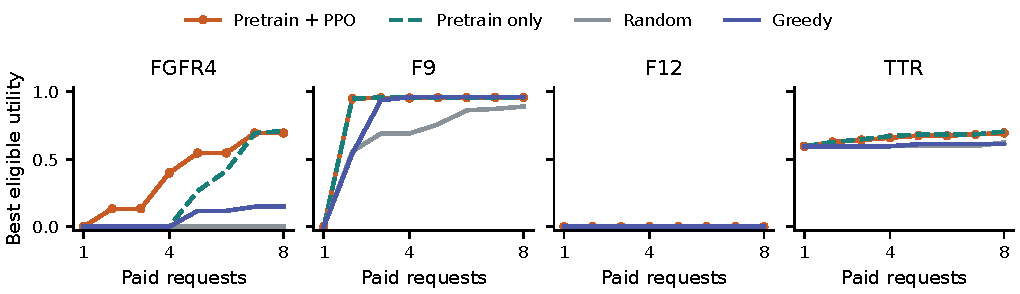
\includegraphics[width=\textwidth]{figures/molecular.pdf}
\caption{Mean best eligible surrogate utility over five policy seeds on four original development targets, at eight charged requests including the starting molecule. Curves are reconstructed from saved query trajectories; overlapping curves are retained. F12's zero outcome is part of the result. Offline training costs are additional and unequal.}
\label{fig:molecular}
\end{figure*}

\begin{table}[t]
\centering
\begin{tabular}{llrrrr}
\toprule
Target &Role&PPO&Pre.&Rand.&Greedy\\
\midrule
DGAT2&T&.888&.888&.409&.487\\
CFB&V&.720&.487&.222&.000\\
FGFR4&D&.694&.709&.000&.148\\
F9&D&.958&.958&.891&.960\\
F12&D&.000&.000&.000&.000\\
TTR&D&.694&.704&.624&.612\\
APOC3&D+&.886&.877&.756&.198\\
ANGPTL3&D+&.926&.926&.795&.614\\
\bottomrule
\end{tabular}
\caption{Eight-request mean surrogate utility. Pre.: staged pretrained policy; Rand.: random search. T: policy training; V: checkpoint validation; D: original development; D+: added development. Predictor exposure also varies, including ANGPTL3. These are not eight independently held-out biological targets.}
\label{tab:molecular}
\end{table}

\section{Discussion}
OLIGARCH connects the studies through a common question: which use of limited information improves the next scientific decision? Prediction studies assess what can be learned; molecular search tests how that knowledge guides proposals; assay replay tests how observations should be purchased. Potency adjudication and concentration stopping examine what those observations establish, while exact planning measures the improvement available under an explicit model. Together, they locate decision value across distinct discovery tasks.

The predictive studies support selective investment. Huesken acquisition improves average learning-curve performance, and Bayesian updates improve predictions as measurements arrive. Yet the tested LoRA adaptations trail classical controls, and improved beliefs do not make PPO the best assay selector. Prediction, uncertainty, and hit yield therefore need separate evaluation: useful measurements change choices or establish required evidence.

The two decision environments expose different costs of sophistication. Molecular pretraining transfers a frozen scorer's preferences into candidate selection; additional PPO uses many more preparation queries for mixed gains. In assay replay, strong rankings already find useful candidates. The synthetic study supplies a way to distinguish limited opportunity for planning from failure to learn: compare against the best attainable expected yield under an assumed model. Near-optimal one-step rollout offers an intermediate control; testing it on calibrated ASO campaign models is a next step.

Measurement studies identify a second route to efficiency. Qualified potency bounds can recover useful evidence without changing a purchase, and fixed stopping can resolve many historical panels with few readouts. The unresolved-panel failure shows that threshold resolution and whole-curve quality require different evidence. Future assay workflows could therefore separate classification from quality verification and reserve additional measurements for ambiguous or questionable panels, with that strategy assessed prospectively rather than tuned to this frozen assessment.

The downstream contribution is a reusable basis for allocating queries and experiments. Assay eligibility, hidden-outcome access, chemical constraints, and expenditure logs let future systems be compared on the decisions they change. The interfaces support eventual laboratory feedback and provide benchmarks for that integration.

\section{Limitations}
Historical Atlas panels reflect patent reporting and prior advancement decisions. Linked follow-up panels are selected populations, missing assays are not negative results, and raw readouts may not represent independent replicates. Exact identity checks leave target aliases, patent families, and broader sequence homology incompletely resolved. Huesken measures siRNA activity, and its split-level acquisition result cannot be generalized to ASO efficacy or safety.

The manuscript spans different cohorts and protocols rather than a single controlled comparison of all algorithms. Reused targets, shared split seeds, and repeated availability draws restrict statistical independence. Atlas source allocations change composition; small target counts restrict inference. Original linked-assay policy records remain unavailable, limiting empirical conclusions for the full screening-to-potency environment.

Molecular search can favor weaknesses in its predictor and propose chemistry or assay conditions outside the training data. There is no certified independent final biological panel for the active design profile, and total offline compute differs across optimizers. The stopping assessment fails its prespecified unresolved-reference criterion; perfect agreement on resolved curves does not rescue that failure or establish a population error bound. Historical full-curve adjudications are imperfect references. The synthetic planning model assumes known observation likelihoods and perfect confirmation, and does not validate uncertainty in real assays.

The evaluations use retrospective measurements and frozen surrogate feedback. Prospective studies should account for plate layout, replication, and fixed setup costs when assessing laboratory efficiency.

\section{Conclusion}
OLIGARCH makes adaptive oligonucleotide discovery testable through two budgeted decision environments and complementary studies of predictive learning, evidence sufficiency, and planning. Uncertainty acquisition and Bayesian updates improve learning, supervised initialization supports effective surrogate search, and conventional ranking and stopping rules provide strong baselines. Exact planning identifies conditions where looking beyond the next reward adds value. Future work should calibrate planning models to measured campaigns, establish independent chemistry-compatible panels, and validate experimental feedback prospectively.

% Review-draft layout requested by the authors; remove this break for camera-ready.
\clearpage
% aaai2027.sty selects its official bibliography style.
\bibliography{references}
\end{document}
